\documentclass{exam}
\usepackage[utf8]{inputenc}
\usepackage{lmodern}
\usepackage{microtype}

% \usepackage[parfill]{parskip}
\usepackage[dvipsnames]{xcolor}
\usepackage{amsmath}
\usepackage{amsfonts}
\usepackage{amsthm}
\usepackage{siunitx}
\DeclareSIUnit\year{yr}
\DeclareSIUnit\foot{ft}
\DeclareSIUnit\litre{\liter}

\usepackage{skull}

\usepackage{pgfplots}
\usepgfplotslibrary{polar}
\pgfplotsset{compat=1.11}
\usepgfplotslibrary{statistics}
\usepackage{graphicx}
\usepackage{sidecap}
\sidecaptionvpos{figure}{c}
\usepackage{float}
\usepackage{gensymb}
\usepackage{tkz-euclide}
\usetkzobj{all}
\usepackage{commath}
\usepackage{hyperref}
\usepackage{enumitem}
\usepackage{wasysym}
\usepackage{multicol}
\usepackage{mathtools}
\usepackage{tcolorbox}
\usepackage{tabularx}
\usepackage[version=4]{mhchem}
\usepackage{changepage}
\usepackage{listings}
\lstset{basicstyle=\ttfamily\linespread{0.8}\small}

\renewcommand*{\thefootnote}{\fnsymbol{footnote}}

\newtheorem*{thm}{Theorem}
\newtheorem*{iden}{Identity}
\newtheorem*{lemma}{Lemma}
\newtheorem{obs}{Observation}
\theoremstyle{definition}
\newtheorem*{defn}{Definition}
\newtheorem*{ex}{Example}
\newtheorem{con}{Construction}
\newtheorem*{alg}{Algorithm}

\newtheoremstyle{break}
  {\topsep}{\topsep}%
  {\itshape}{}%
  {\bfseries}{}%
  {\newline}{}%
\theoremstyle{break}
\newtheorem*{bthm}{Theorem}

% russian integral
\usepackage{scalerel}
\DeclareMathOperator*{\rint}{\scalerel*{\rotatebox{17}{$\!\int\!$}}{\int}}

% \DeclareMathOperator*{\rint}{\int}

\pgfplotsset{vasymptote/.style={
    before end axis/.append code={
        \draw[densely dashed] ({rel axis cs:0,0} -| {axis cs:#1,0})
        -- ({rel axis cs:0,1} -| {axis cs:#1,0});
    }
}}

% \pointsinrightmargin
\boxedpoints
\pointname{}

\newcommand{\questioA}{\question[\texttt{\textbf{\color{Cerulean} A}}]}
\newcommand{\questioM}{\question[\texttt{\textbf{\color{PineGreen} M}}]}
\newcommand{\questioE}{\question[\texttt{\textbf{\color{WildStrawberry} E}}]}
\newcommand{\questioS}{\question[\texttt{\textbf{\color{Goldenrod} S}}]}
\newcommand{\questioO}{\question[\texttt{\textbf{\color{BurntOrange} O}}]}

\newcommand{\parA}{\part[\texttt{\textbf{\color{Cerulean} A}}]}
\newcommand{\parM}{\part[\texttt{\textbf{\color{PineGreen} M}}]}
\newcommand{\parE}{\part[\texttt{\textbf{\color{WildStrawberry} E}}]}
\newcommand{\parS}{\part[\texttt{\textbf{\color{Goldenrod} S}}]}
\newcommand{\parO}{\part[\texttt{\textbf{\color{BurntOrange} O}}]}

\newcommand{\subparA}{\subpart[\texttt{\textbf{\color{Cerulean} A}}]}
\newcommand{\subparM}{\subpart[\texttt{\textbf{\color{PineGreen} M}}]}
\newcommand{\subparE}{\subpart[\texttt{\textbf{\color{WildStrawberry} E}}]}
\newcommand{\subparS}{\subpart[\texttt{\textbf{\color{Goldenrod} S}}]}
\newcommand{\subparO}{\subpart[\texttt{\textbf{\color{BurntOrange} O}}]}

\newcommand{\mainHeader}[2]{\section*{NCEA Level 2 Mathematics\\#1. #2}}
\newcommand{\mainHeaderHw}[2]{\section*{NCEA Level 2 Mathematics (Homework)\\#1. #2}}
\newcommand{\seealso}[1]{\begin{center}\emph{See also #1.}\end{center}}
\newcommand{\drills}[1]{\begin{center}\emph{Drill problems: #1.}\end{center}}
\newcommand{\basedon}[1]{\begin{center}\emph{Notes largely based on #1.}\end{center}}

\begin{document}

\mainHeaderDiff{12}{Kinematics}
\textcolor{orange}{\textbf{This is an easy week, especially if you are doing physics (or did level 2 physics). Take a well-earned break!}}
Calculus was independently developed by Sir Isaac Newton to describe motion in physics. This use is known as \textit{kinematics} (from the
Greek \textit{kinein}, `to move'). Suppose a particle moves from position $ x_0 $ to position $ x_1 $ over a time $ \Delta t $. We call the
ratio
\begin{displaymath}
  \frac{x_1 - x_0}{\Delta t}
\end{displaymath}
the \textit{average velocity} of the particle; if we let $ x_1 \to x_2 $, we obtain the derivative $ \od{x}{t} = v $, the \textit{instantaneous
velocity} of the particle at the point $ x $ (usually just abbreviated to velocity).

Similarly, the rate of change of velocity is called \textit{acceleration}. We have $ a = \od{v}{t} $.

\begin{center}
  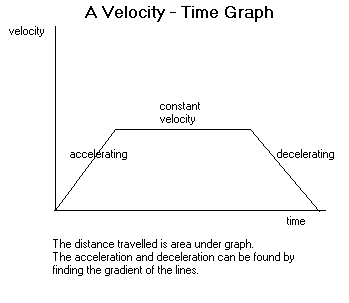
\includegraphics[width=0.5\linewidth]{vgraph}
\end{center}
If we draw a velocity-time graph, like that above, the area under the graph gives us the distance travelled by the object
during a time interval; this means that in some sense finding area is inverse to finding slope. Intuitively, this is a bit
weird --- the way to think about it is that if we increase the area under the velocity curve by a little bit, then the distance
we move in that time also increases proportionally. On the other hand, if we move a certain distance then we increase the area
under the velocity curve because we have a non-zero velocity.

Algebraically, we have $ \text{rate} = \frac{\text{change in quantity}}{\text{time}} $ and so $ \text{change in quantity} = \text{rate} \times \text{time} $.

We will explore this idea in more detail in a couple of weeks when we start talking about \textit{integration}.

We can derive the following \textit{kinematic equations} if acceleration is kept constant over a time period $ t $:
\begin{align*}
  v_f &= v_i + a \Delta t\\
  \Delta x &= v_i \Delta t + \frac{1}{2} a {\Delta t}^2\\
  v_f^2 &= v_i^2 + 2a \Delta x\\
  \Delta x &= \frac{v_f + v_i}{2} \Delta t
\end{align*}

These can all be found from the definitions of acceleration and velocity, and by taking areas and slopes of graphs (if
we remember that the velocity graph must be made up of straight lines since the acceleration is constant). The equations
are not examinable in the L3 calculus exam. We mainly look at them for context.

\subsection*{Questions}
All distances are given in \si{\metre}, and all times in \si{\second}, unless otherwise stated.
\begin{questions}
  \questioA Describe the relationship between velocity and displacement.
  \questioA A particle moves from $ x = \SI{2}{\metre} $ to $ x = \SI{3}{\metre} $ over a time \SI{3}{\second}. What is its average velocity over that time?
  \questioA A particle moves from $ (3,4) $ to $ (12,-3) $ over a time \SI{10}{\second}. If the displacements are measured in metres, what is the magnitude of
            its average velocity during that period?
  \questioA An object $ A $ has a positive acceleration $ a $, and a second object $ B $ has a negative acceleration $ -a $. Both are moving in the
            same direction. Which of the following is \textbf{not} true?
    \begin{parts}
      \part Object $ B $ is slowing down compared to object $ A $.
      \part Object $ B $ has a lower velocity than object $ A $.
      \part At some point, object $ B $ will reach a velocity of zero and then start moving in the opposite direction.
      \part If object $ B $ is behind object $ A $, the two will never cross paths.
    \end{parts}
  \questioA Suppose a particle has a velocity of $ \SI{34}{\metre\per\second} $. How long does it take for the particle to travel \SI{150}{\metre}?
  \question The velocity $ v $ of an object $ t $ seconds after it moves from the origin is given by
            \begin{displaymath}
              v(t) = 3t^2 - 6t - 24.
            \end{displaymath}
    \begin{parts}
      \parA Write down the formulae for the acceleration of the particle after $ t $ seconds.
      \parA Work out the initial velocity and acceleration.
      \parA When is the object at rest momentarily?
      \parM When is the object travelling at minimum speed?
      \parM When did the object return to the origin?
    \end{parts}
  \questioA A well-wrapped food parcel is dropped from an aeroplane flying at a height of \SI{500}{\metre}
            above the ground. The constant acceleration due to gravity is \SI{-9.81}{\metre\per\second\squared}. Air resistance
            is negligible.
    \begin{parts}
      \part How long does it take for the food parcel to hit the ground?
      \part How fast is the food parcel moving when it hits the ground?
    \end{parts}
  \questioA A racing car travelling at \SI{210}{\kilo\metre\per\hour} skids for a distance of \SI{150}{\metre}
            after its brakes are applied. The brakes provide a constant deceleration.
    \begin{parts}
      \part What is the deceleration in \si{\metre\per\second\squared}?
      \part How long does it take for the car to stop?
    \end{parts}
  \questioE The displacement of an object moving in a straight line on either side of a fixed origin is given by
            \begin{displaymath}
              s(t) = 2t^3 - 12t^2 + 18t + 3.
            \end{displaymath}
            Find the minimum velocity of the object. Prove that it is a minimum. Which position is it at at that time?
  \questioM Derive the kinematic equations by looking at the velocity graph of an object with constant acceleration.
\end{questions}
\end{document}
